\section{Взаимодействие среды исполнения смарт-кон\-трак\-тов с \name{Hy\-per\-led\-ger Iro\-ha}}
В этой главе будет рассмотрена схема взаимодействия среды исполнения смарт-контрактов и программный интерфейс, который эту схему реализует.

\subsection{Схема взаимодействия}
\label{Interaction}

\begin{figure}[b!]
  \centering
  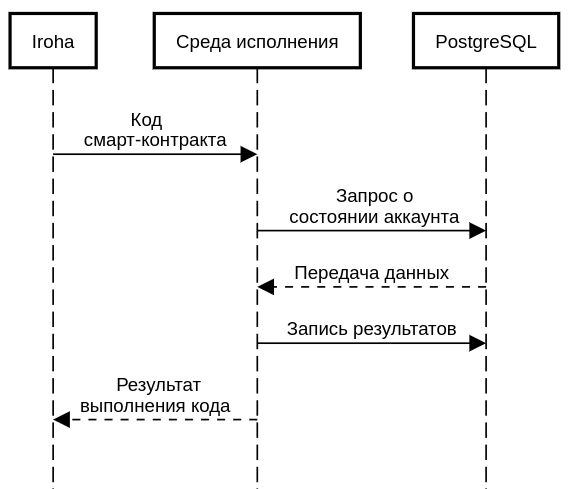
\includegraphics[width=0.6\columnwidth]{interaction.png}
  \caption{Диаграмма последовательности взаимодействия}
  \label{interaction}
\end{figure}

Для создания инфраструктуры для среды исполнения смарт-кон\-трак\-тов необходимо разработать схему взаимодействия этой среды и блокчейна \name{Hy\-per\-led\-ger Iro\-ha}.
Среда исполнения должна уметь получать и записывать данные в блокчейн.

На рисунке~\ref{interaction} показано взаимодействие среды исполнения с \name{Hy\-per\-led\-ger Iro\-ha} и локальной базой данных \name{PostgreSQL}, в которой хранится история транзакций, права доступа и информация о пользователях.
Среда исполнения принимает на вход код смарт-контракта и начинает его выполнение.
Для того, чтобы получать и записывать актуальное состояние переменных смарт-контракта, среда исполнения обращается к базе данных.
Запросы выполняются по необходимости.

\subsection{Реализация интерфейса взаимодействия}
\label{AddSmartContract}
Пользователи формируют транзакции с помощью специального набора команд.
Для работы с командами в коде используется паттерн <<фабричный метод>>.
Для того, чтобы участники могли сохранять и выполнять код смарт-контракта, была добавлена новая команда \emph{Add\-Smart\-Con\-tract}.
Она содержит в себе данные, необходимые для вызова среды исполнения.
То, что будет передано, зависит от конкретной среды исполнения.
Для передачи транзакций и записи в блокчейн используются библиотеки \name{Protobuf} и \name{RapidJSON}, поэтому нужно уметь переводить данные, содержащиеся в AddSmartContract (как и в любой другой команде), в форматы \name{Protocol Buffers} и \name{JSON} и обратно во внутреннее представление.

Перед тем, как транзакция будет записана в истории блокчейна, все участники сети должны провести stateless и stafeful валидацию всех команд внутри этой транзакции.
Для AddSmartContract stateless валидация может содержать различные проверки кода, например на синтаксическую корректность.
Во время stateful валидации участник сети обязан выполнить код и получить новое состояние блокчейна, чтобы в дальнейшем во время работы алгоритма консенсуса все участники договорились, принимать это новое состояние или нет.

\vspace{0.7cm}
\noindent\achtung{Таким образом, было достигнуто то-то с такими-то свойствами}
